\documentclass[10pt]{beamer}
\usetheme{Warsaw}
\usepackage[T1]{fontenc}
\usepackage[utf8]{inputenc}
\usepackage{chronosys}
\usepackage{graphicx}
\usepackage{stmaryrd}
\usepackage{float}
\usepackage{caption}
\title{Kinetic}
\author[Demuth Axel, Geraldes Pereira Dorian]{Team member: \newline\newline Demuth Axel \newline Geraldes Pereira Dorian \newline\newline Supervisor :  \newline\newline Pierre Alliez \newline Vincent Chabannes}
\date{}
\begin{document}
\frame{\titlepage}
\begin{frame}
    \tableofcontents
\end{frame}
\section{Introduction}

\begin{frame}{Context}
\end{frame}
\begin{frame}{Objectives}
\begin{itemize}
    \item \textbf{Reading Process and Mesh Conversion: }Convert data from stl file to ply and xyz file with normals on points
    
    \item \textbf{Application of the Kinetic Algorithm}
    
    \item \textbf{Recovery of Material Labels}
    
    \item \textbf{Utilization on City Modeling}
\end{itemize}
\end{frame}
\begin{frame}{Challenges}
\begin{itemize}    
    \item \textbf{Generating point cloud from stl file}
\begin{figure}[H]
        \begin{minipage}[t]{0.25\textwidth}
            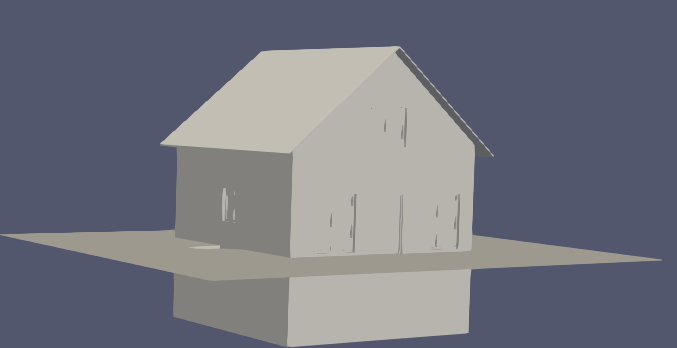
\includegraphics[width=\textwidth]{../../images/screen_kinetic/ACJasmin.png}
            \caption*{ACJasmin stl}
        \end{minipage}
        \begin{minipage}[t]{0.20\textwidth}
          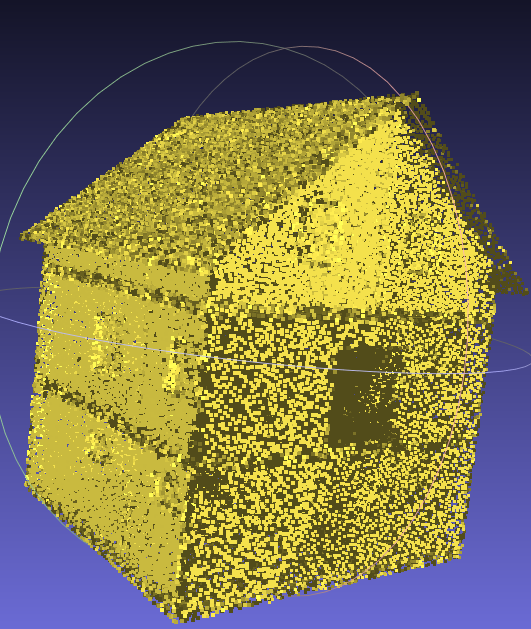
\includegraphics[width=\textwidth]{../../images/screen_kinetic/ACJasmin_point_cloud.png}
          \caption*{ACJasmin point cloud}
        \end{minipage}
\end{figure}
    \item \textbf{Parameter Optimization}
\end{itemize}
\end{frame}

\section{Tools}
\begin{frame}{Cgal}
    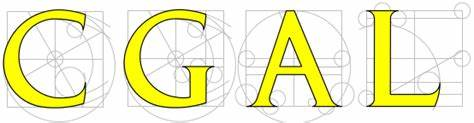
\includegraphics[scale = 0.2]{../../images/CGAL_logo.png}
    \begin{itemize}
        \item C++ library for geometric calcul 
        \item Provides data structures and algorithms for:
        \begin{itemize}
            \item Computational geometry
            \item Mesh generation and processing
            \item Geometry processing
            \item Surface and volume manipulation
        \end{itemize}
        \item For our usage Kinetic surface reparation algorithme, file reader
    \end{itemize}

\end{frame}{Kinetic}
Kinetic algorithm is an geometric algorithm to work on 3D mesh it uses  geometric primitive with an energy based model to fit the primitives to the model.

Energy formule: 
\newline
\begin{center}
    $        U(x) = w_f U_f(x) + w_s U_c(x) + w_c U_c(x)       $
\end{center}

to calculate the best primitive to fit the mesh.
then we have a list of geometric operation on each primitive
\begin{itemize}
    \item merging
    \item splitting 
    \item transfer 
    \item insertion
    \item exclusion
\end{itemize}

\begin{frame}
Here the speudo code of the application of geometric application : 
\begin{center}
    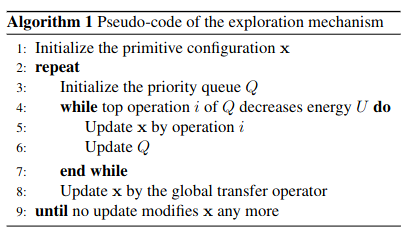
\includegraphics[scale =  0.5]{../../images/Pseudo_code_exploration.png}
  \end{center} 
\end{frame}


\section{Implementation}
\begin{frame}{STL (STereoLithography)}
    \begin{itemize}
        \item File format for 3D modeling
        \item Stock a collection of triangle composing the mesh without any other information
    \end{itemize}
    \begin{center}
        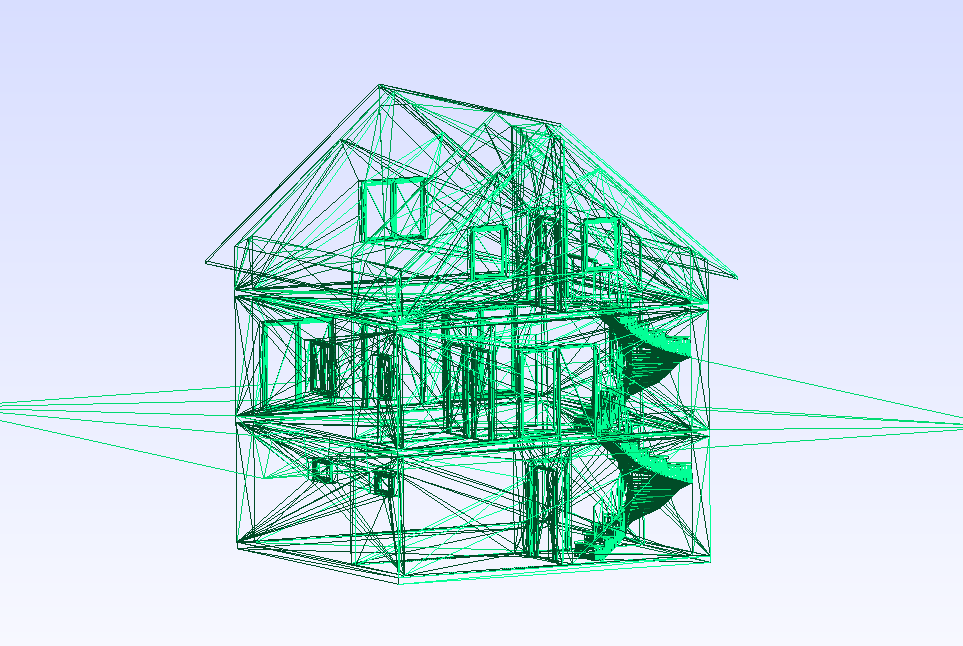
\includegraphics[scale=0.3]{../../images/ACJASMINSTL.png}
    \end{center}
\end{frame}

\section{Analysis of Result}
\begin{frame}{first result}
First we can show you what KSR algorithm is capable of: 
\begin{figure}[H]
    \begin{minipage}[t]{0.29\textwidth}
        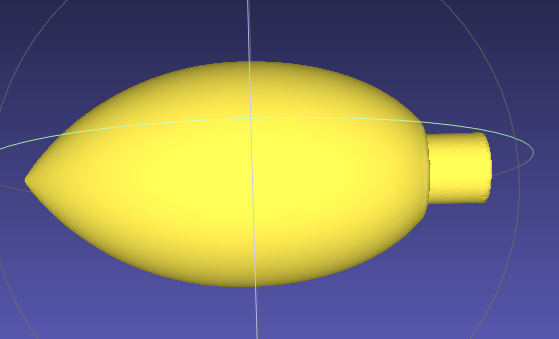
\includegraphics[width=\textwidth]{../../images/screen_kinetic/flame_point.png}
        \caption*{flame point cloud}
    \end{minipage}
    \begin{minipage}[t]{0.29\textwidth}
      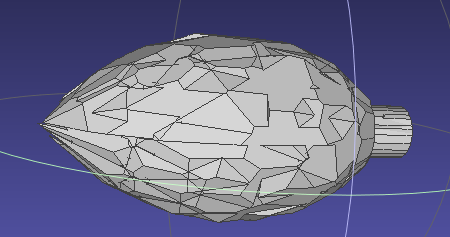
\includegraphics[width=\textwidth]{../../images/screen_kinetic/flame_cgal.png}
      \caption*{flame with cgal}
    \end{minipage}
    \begin{minipage}[t]{0.29\textwidth}
        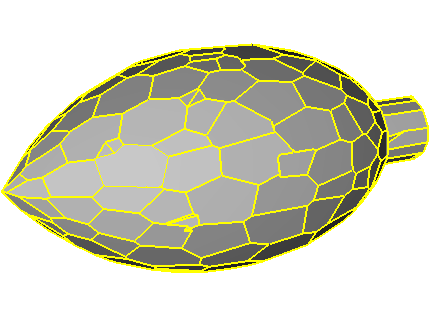
\includegraphics[width=\textwidth]{../../images/screen_kinetic/flame_inria.png}
        \caption*{flame with inria}
      \end{minipage}
\end{figure}
\end{frame}
\subsection*{first example}
\begin{frame}{conversion to point cloud}
    \begin{figure}[H]
        \centering
        \begin{minipage}[t]{0.35\textwidth}
          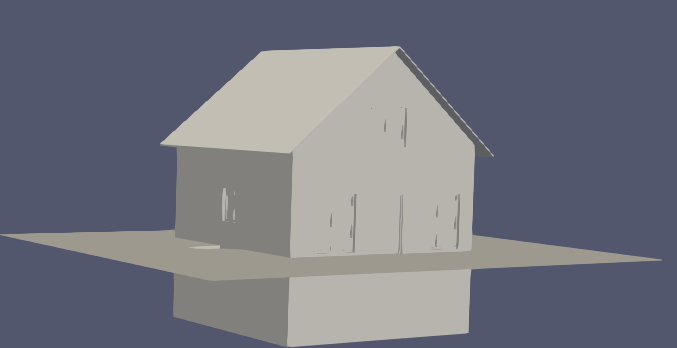
\includegraphics[width=\textwidth]{../../images/screen_kinetic/3zones.png}
          \caption*{3zones}
        \end{minipage}
        \begin{minipage}[t]{0.35\textwidth}
            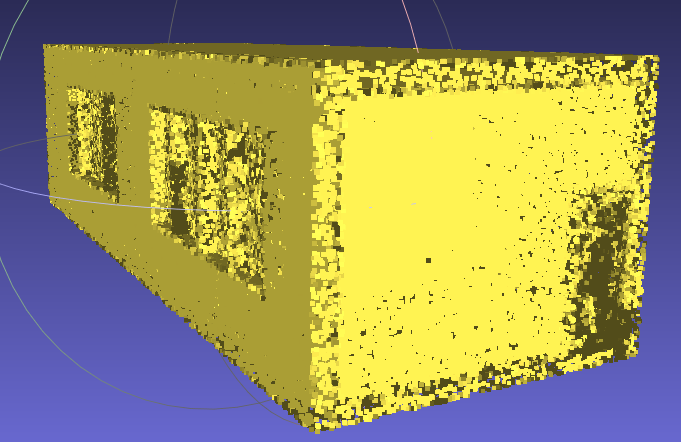
\includegraphics[width=\textwidth]{../../images/screen_kinetic/3zones_point_cloud.png}
            \caption*{3zones point cloud}
          \end{minipage}
      \end{figure}  
\end{frame}
\begin{frame}{result}
    \begin{figure}[H]
        \centering
        \begin{minipage}[t]{0.45\textwidth}
          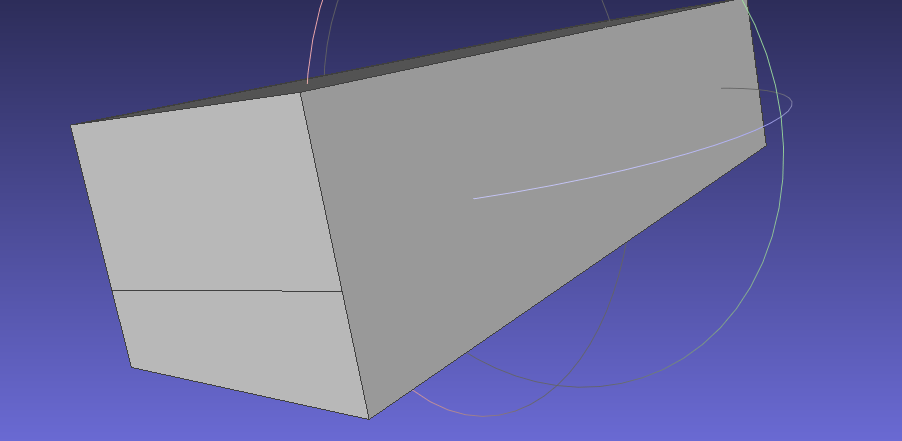
\includegraphics[width=\textwidth]{../../images/screen_kinetic/3zones_result_normal5_cgal.png}
          \caption*{3zones result with normal by Meshlab}
        \end{minipage}
        \begin{minipage}[t]{0.35\textwidth}
            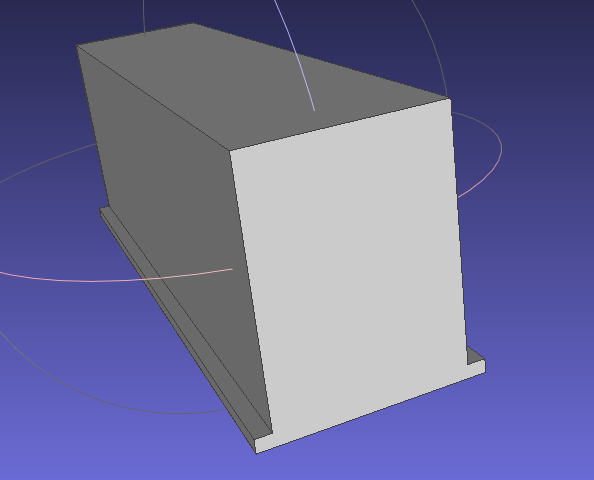
\includegraphics[width=\textwidth]{../../images/screen_kinetic/3zones_result_normal_cgal.png}
            \caption*{3zones result with normal by Cgal}
          \end{minipage}
      \end{figure}  
\end{frame}
\subsection*{second example}
\begin{frame}{conversion to point cloud }
    \begin{figure}[H]
        \centering
        \begin{minipage}[t]{0.40\textwidth}
          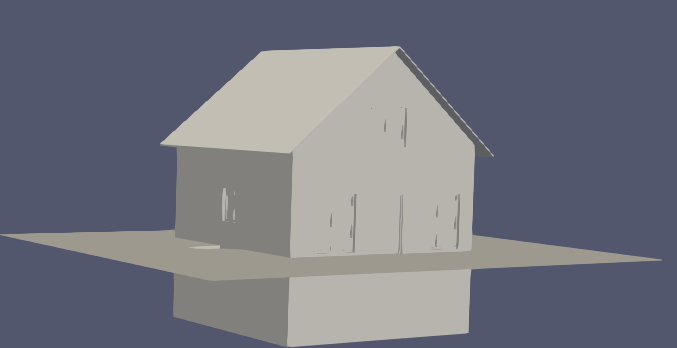
\includegraphics[width=\textwidth]{../../images/screen_kinetic/ACJasmin.png}
          \caption*{ACJasmin}
        \end{minipage}
        \begin{minipage}[t]{0.35\textwidth}
            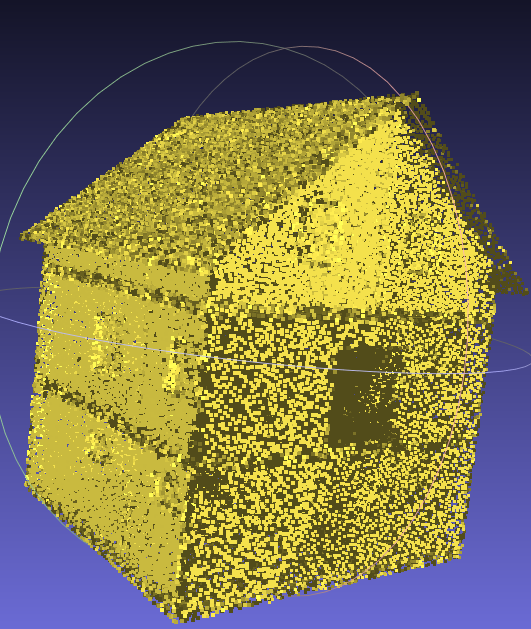
\includegraphics[width=\textwidth]{../../images/screen_kinetic/ACJasmin_point_cloud.png}
            \caption*{ACJasmin point clouds}
          \end{minipage}
      \end{figure}  
\end{frame}
\begin{frame}{cgal kinetic result }
    \begin{figure}[H]
        \centering
        \begin{minipage}[t]{0.29\textwidth}
          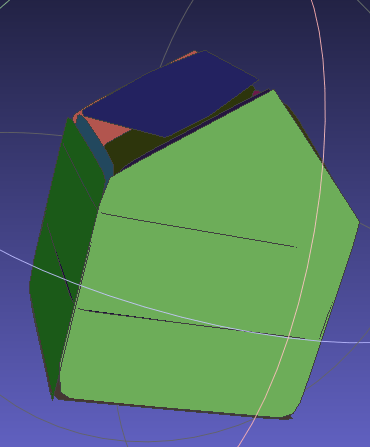
\includegraphics[width=\textwidth]{../../images/screen_kinetic/ACJasmin_primitive_cgal.png}
          \caption*{ACJasmin primitives by Cgal}
        \end{minipage}
        \begin{minipage}[t]{0.35\textwidth}
            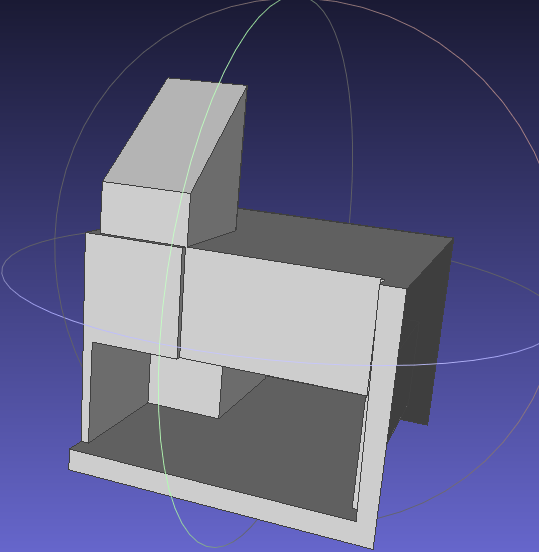
\includegraphics[width=\textwidth]{../../images/screen_kinetic/ACJasmin_result_CGAL.png}
            \caption*{ACJasmin result with Cgal}
          \end{minipage}
      \end{figure}  
\end{frame}
\begin{frame}{INRIA kinetic result }
    \begin{figure}[H]
        \centering
        \begin{minipage}[t]{0.29\textwidth}
          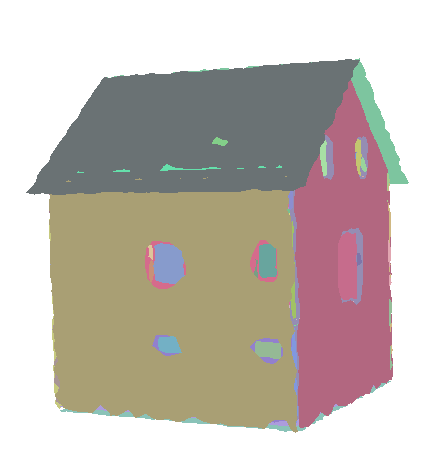
\includegraphics[width=\textwidth]{../../images/screen_kinetic/ACJasmin_primitive.png}
          \caption*{ACJasmin primitives by INRIA}
        \end{minipage}
        \begin{minipage}[t]{0.35\textwidth}
            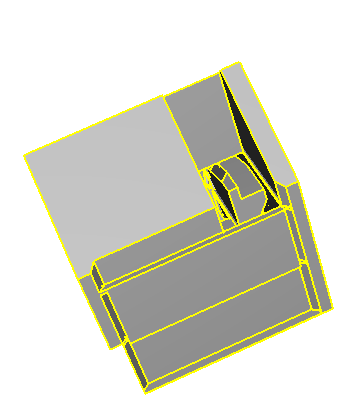
\includegraphics[width=\textwidth]{../../images/screen_kinetic/ACJasmin_result_INRIA.png}
            \caption*{3zones result with INRIA}
          \end{minipage}
      \end{figure}  
\end{frame}


\begin{frame}[allowframebreaks]{reference}
    \nocite{*}
    \bibliographystyle{unsrt}
    \bibliography{../../bibliography/vfinal/report_bib}
\end{frame}

\end{document}